\subsubsection{Instancias con soluciones no óptimas}
\subsubsubsection{Ver más allá}
Por la naturaleza de la heurística y como veremos en la experimentación, $Savings$ suele dar una solución eficiente. Sin embargo, sigue siendo una heurística y no es seguro que de valores cercanos a la solución óptima. Como ya mencionamos, no es fácil resolver este problema exactamente por lo que una aproximación a la solución es una buena idea: savings podría dar una muy buena solución inicial y a partir de ella, ser mejorada con técnicas computacionales o incluso por humanos. Es interesante esta idea, ya que en ciertos casos a veces tendemos a imaginar que el algoritmo debería ver ``mas allá'', al igual que el ojo humano. Por eso, una persona podría encontrar una mejora en los caminos propuestos por una heurística con facilidad.
\par 
El concepto de ``no ver a futuro'' es lo que hace que savings pueda tener malos casos. Recorre las posibles conexiones de nodos que producen la mayor ganancia en distancia pero eligiéndolas siempre que puede. Es decir, si la ruta es factible y el camión que la recorre tiene la capacidad suficiente, el respectivo saving es elegido, las rutas mergeadas, los nodos conectados. En consecuencia, cada opción tomada restringirá a las siguientes. El caso obvio de esto son las restricciones de capacidad pero no tenemos que olvidar que para poder usar la conexión de dos nodos ninguno puede ser un nodo interno (en ese caso, ya fue conectado a dos vecinos y como son caminos hamiltonianos, no es posible la unión con un tercero). A partir de esto surge el razonamiento de que ocurriría si se saltea un saving pensando a futuro.  
\par 
Esta es la idea del algorítmo de \textbf{Holmes and Parker}, cuyo principio es permitir la prohibición de conexiones (que aunque tengan valor alto de saving) afecten las posibles conexiones siguientes. De esta forma, se forma un árbol de posibles soluciones con cada decisión tomada y se elige la mejor. Las condición para parar podrían depender de hasta que punto estamos dispuestos a explorar, el tamaño del árbol, etc.
\subsubsubsection{Rutas circulares}
El efecto inmediato de lo mencionado anteriormente es que una conexión no pueda ser deseleccionada. Por lo tanto, sobre todo cuando la capacidad es ajustada, savings suele armar cierto tipo de rutas, periféricas, circulares. 
\par 
Más específicamente, tomamos instancias donde no da una solución óptima y la comparamos con ella.
\begin{figure}[H]
	\centering
	\begin{minipage}{0.35\textwidth}
		\centering
		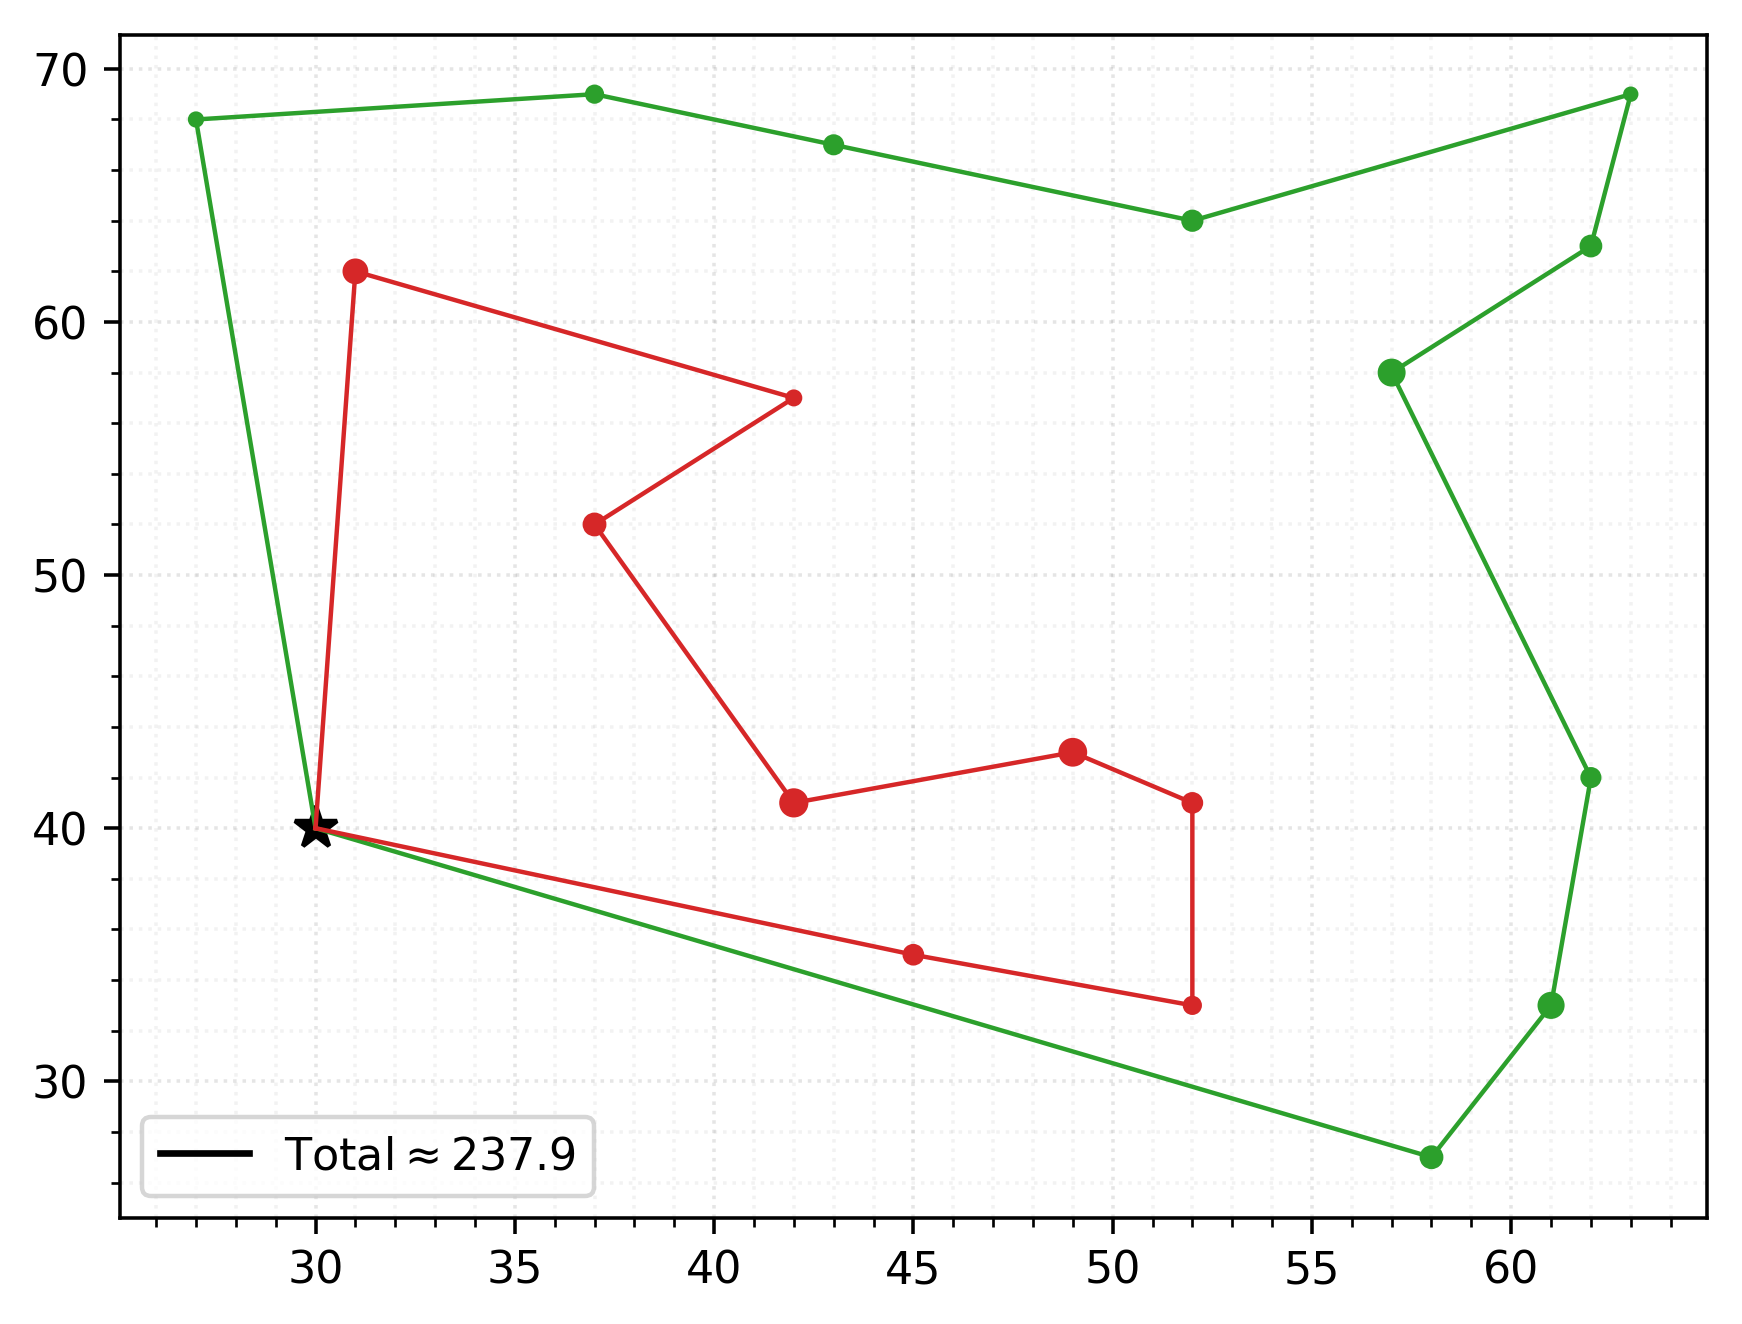
\includegraphics[width=1\textwidth]{images/savings/malosavingchico2}
		\caption{\footnotesize Ruta resultado savings para la instancia \textbf{P-n19-k2}}
		\label{fig:savings-malo-chico2}
	\end{minipage}%
	\hspace{0.03\textwidth}
	\begin{minipage}{0.35\textwidth}
		\centering
		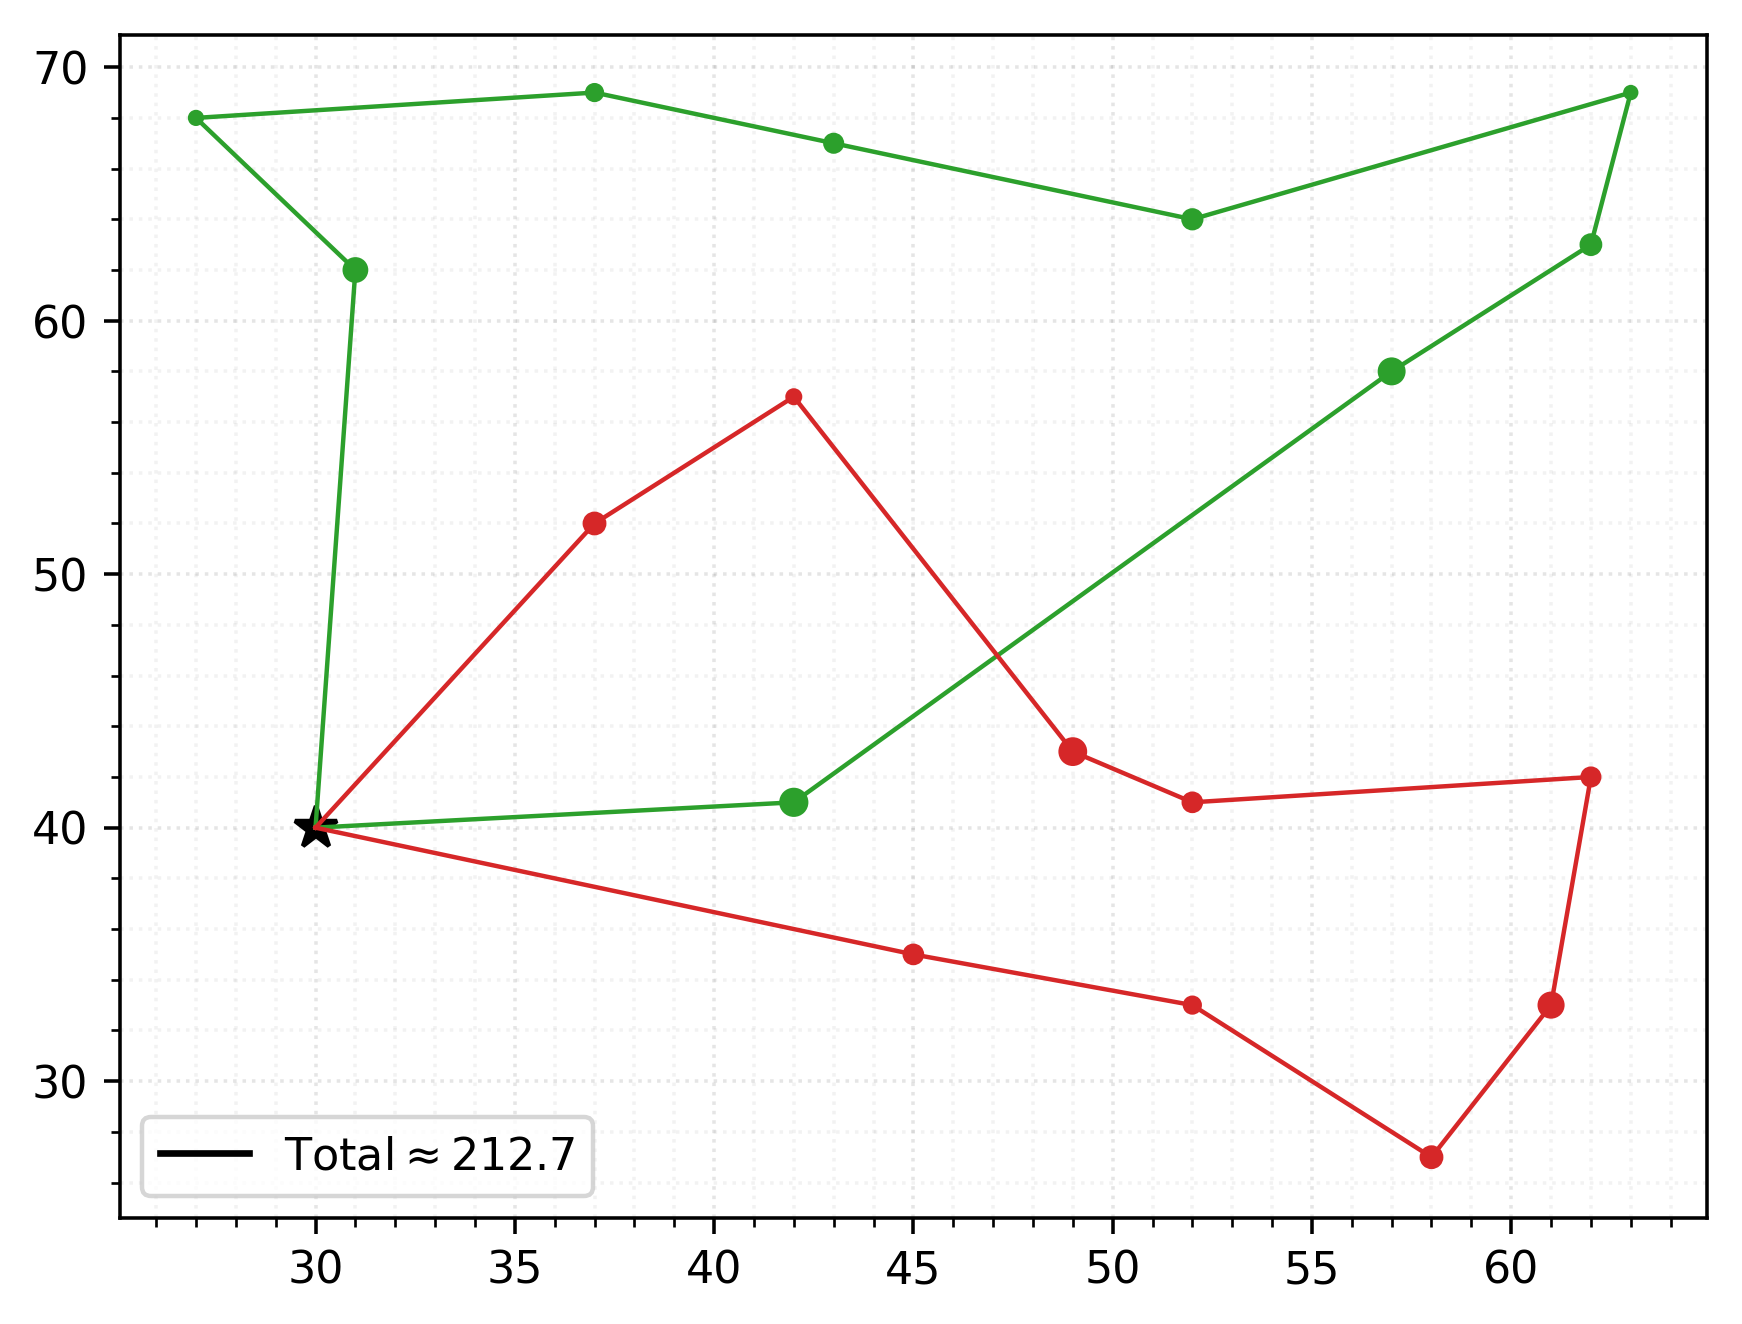
\includegraphics[width=1\textwidth]{images/savings/optimochico2}
		\caption{\footnotesize Ruta óptima para la instancia \textbf{P-n19-k2}}
		\label{fig:savings-optimo-chico2}
	\end{minipage}%
\end{figure}
\begin{figure}[H]
	\centering
	\begin{minipage}{0.35\textwidth}
		\centering
		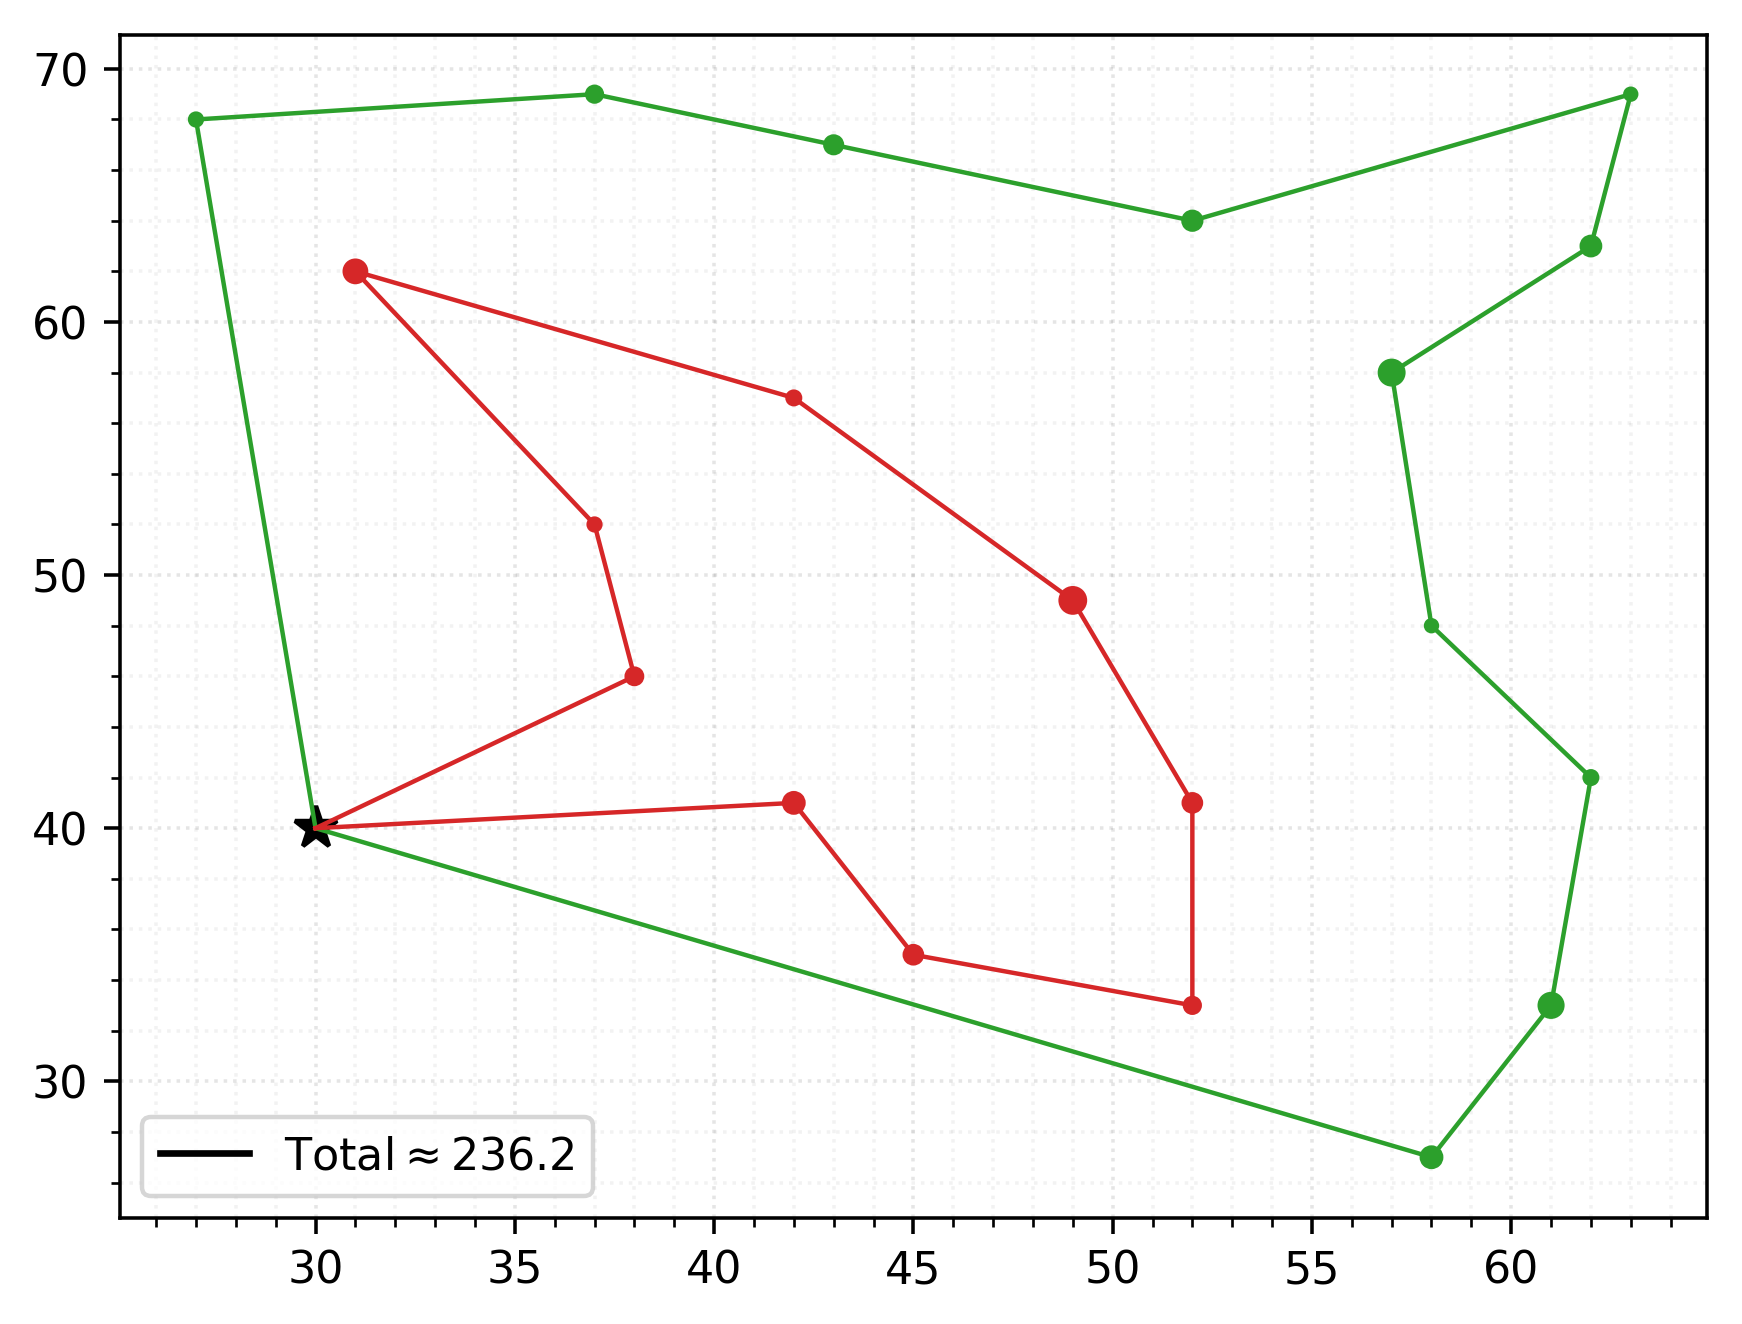
\includegraphics[width=1\textwidth]{images/savings/malosavingchico}
		\caption{\footnotesize Ruta resultado savings para la instancia \textbf{P-n21-k2}}
		\label{fig:savings-malo-chico}
	\end{minipage}%
	\hspace{0.03\textwidth}
	\begin{minipage}{0.35\textwidth}
		\centering
		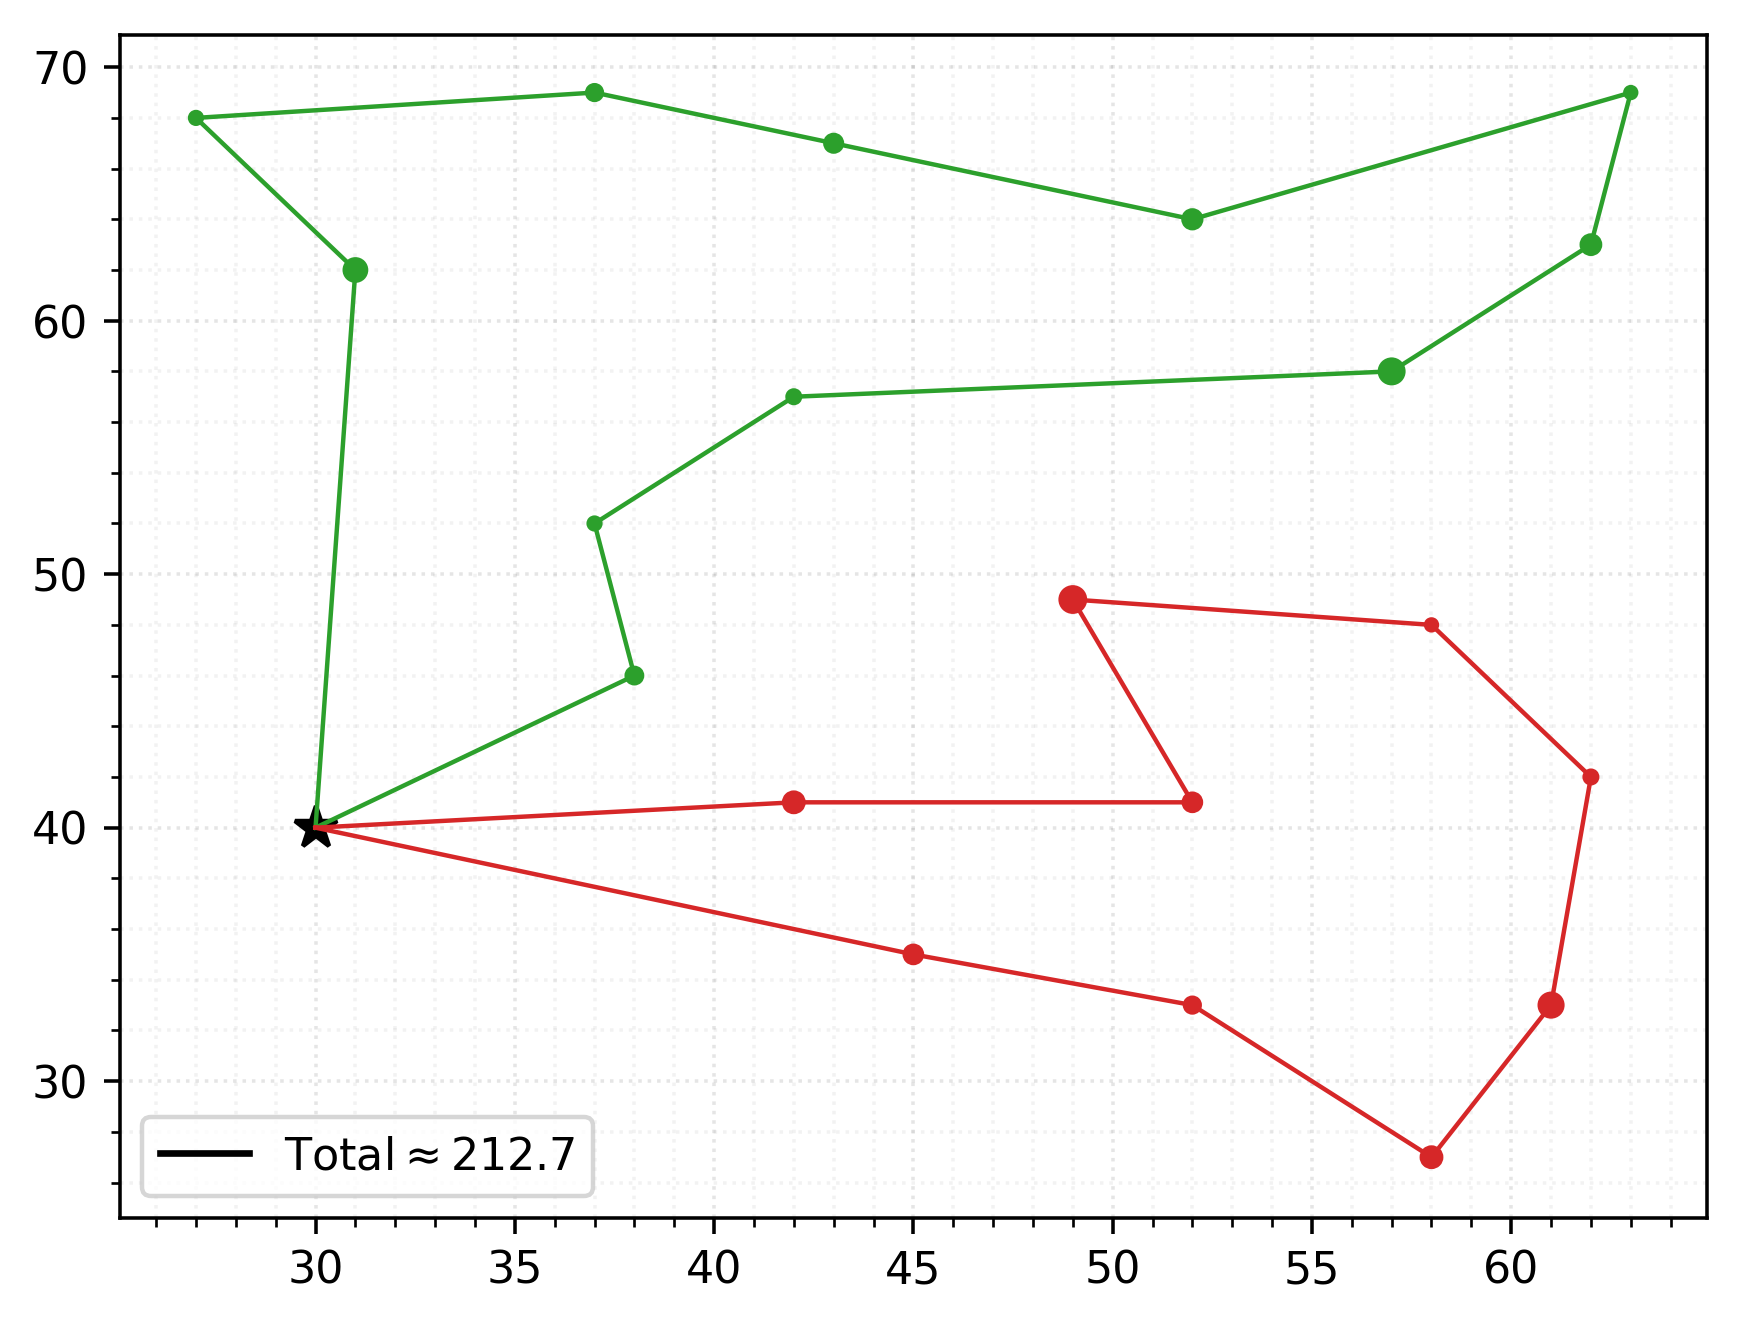
\includegraphics[width=1\textwidth]{images/savings/optimochico}
		\caption{\footnotesize Ruta óptima para la instancia \textbf{P-n21-k2}}
		\label{fig:savings-optimo-chico}
	\end{minipage}%
\end{figure}
Si bien las soluciones óptimas tienen una forma de ruta distinta entre sí, podemos notar que saving en ambos casos dio esta forma de ruta. 
\par Otro caso que pertenecerá al mismo data set que los últimos dos, con los que experimentaremos luego es el de la figura \ref{fig:savings-malo-grande}. Aquí es más marcada la diferencia entre ambos recorridos, siendo savings un 15.2\% peor que la óptima.
\begin{figure}[H]
	\centering
	\begin{minipage}{0.35\textwidth}
		\centering
		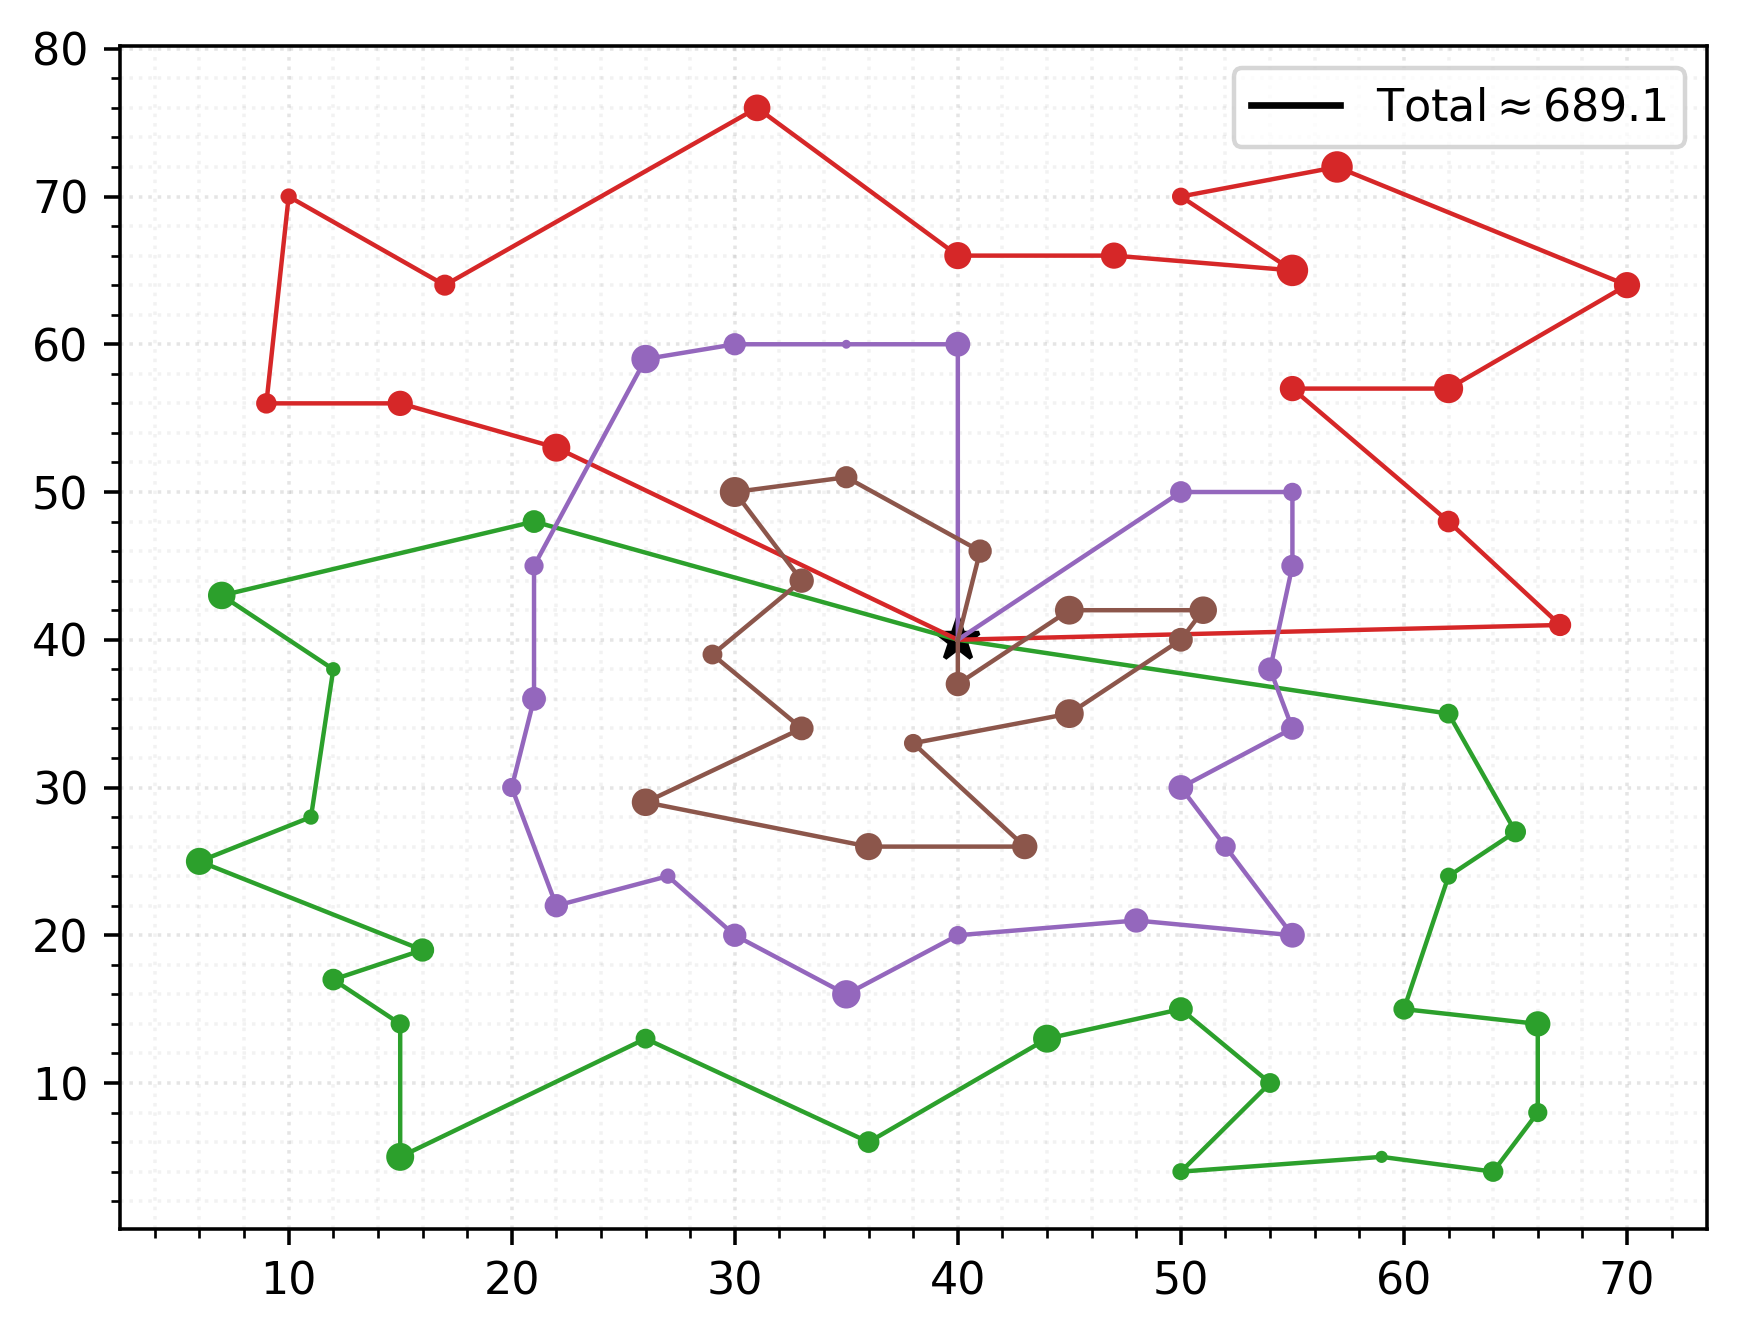
\includegraphics[width=1\textwidth]{images/savings/malosavinggrande}
		\caption{\footnotesize Ruta resultado savings para la instancia \textbf{P-n76-k4}}
		\label{fig:savings-malo-grande}
	\end{minipage}%
	\hspace{0.03\textwidth}
	\begin{minipage}{0.35\textwidth}
		\centering
		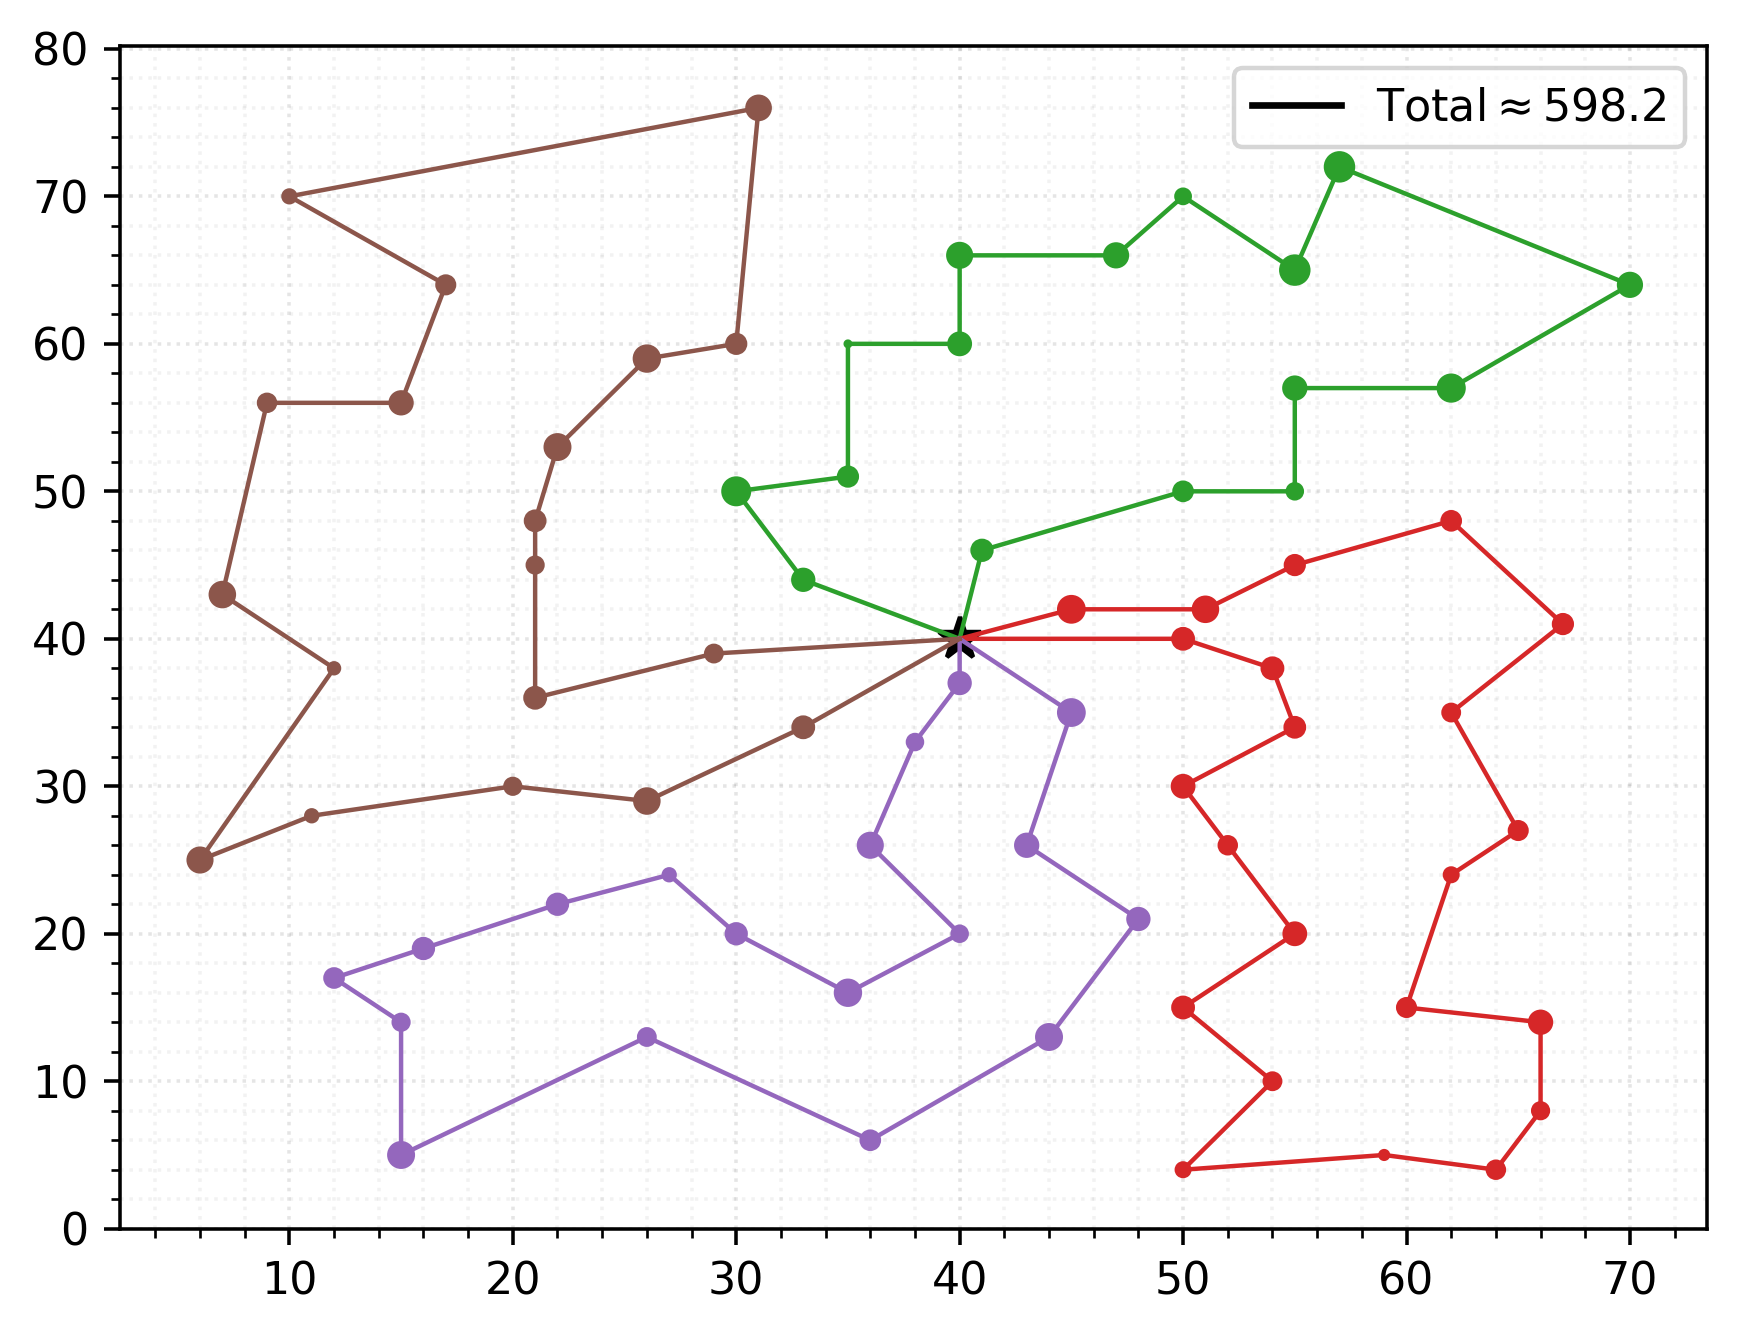
\includegraphics[width=1\textwidth]{images/savings/optimogrande}
		\caption{\footnotesize Ruta óptima para la instancia \textbf{P-n76-k4}}
		\label{fig:savings-optimo-grande}
	\end{minipage}%
\end{figure}

